
\subsection{O Envelope} % (fold)
\label{sub:o_envelope}

\subsubsection{Gás do Balão}

	Existem duas possibilidades para a escolha do gás do balão cativo, o gás hélio e o gás hidrogênio. A seguir são apresentadas duas tabelas contendo as características físicas dos gases que podem ser escolhidos para o balão. Nas tabelas \ref{tab:caracHelio} e \ref{tab:caracHidro} as características do hélio e do hidrogênio são tiradas da empresa \textit{Gama Gases}.

	\begin{table}[H]
		\centering
		\begin{tabular}{|c|c|}
			\hline
			\rowcolor[HTML]{FFFFFF}
			{\color[HTML]{000000} \textbf{Propriedades}}          & {\color[HTML]{000000} \textbf{Valores Numéricos}}                                    \\ \hline
			Densidade absoluta, gás a 101,325kPa a 0 ºC.           & 0,1785 $Kg/m^3$                                                                         \\ \hline
			Densidade crítica                                     & 0,5307 $Kg/m^3$                                                                       \\ \hline
			Densidade relativa, gás a 101,325 kPa a 0 ºC,(ar = 1). & 0,138                                                                                \\ \hline
			Fator crítico de compressibilidade                    & 0,305                                                                                \\ \hline
			Fórmula                                               & 4He                                                                                  \\ \hline
			Massa Molecular                                       & 4,002602                                                                             \\ \hline
			Pressão crítica                                       & \begin{tabular}[c]{@{}c@{}}229 kPa ; 2,29 bar; 33,2 \\ psia;,2,261 atm.\end{tabular} \\ \hline
			Viscosidade, gás a 101,325 kPa a 26,8 ºC.              & 0,02012 mPa x s; 0,02012 cP.                                                         \\ \hline
			Volume específico a 21,1 ºC 101,325 kPa                & 6030,4 dm3/ kg; 96,6 ft3/ Ib                                                         \\ \hline
		\end{tabular}
		\caption[Características do Hélio]{Características do Hélio\cite{gamagases1}}
		\label{tab:caracHelio}
	\end{table}


\begin{table}[H]
	\centering
	\begin{tabular}{|c|c|}
		\hline
		\rowcolor[HTML]{FFFFFF}
		{\color[HTML]{000000} \textbf{Propriedades}}          & {\color[HTML]{000000} \textbf{Valores Numéricos}}                                     \\ \hline
		Densidade absoluta, gás a 101,325kPa a 0ºC.           & 0,08235 $Kg/m^3$                                                                         \\ \hline
		Densidade crítica                                     & 0,0310 $Kg/m^3$                                                                         \\ \hline
		Densidade relativa, gás a 101,325 kPa a 0ºC,(ar = 1). & 0,0695                                                                                \\ \hline
		Fator crítico de compressibilidade                    & 0,305                                                                                 \\ \hline
		Fórmula                                               & H2                                                                                    \\ \hline
		Limites de inflamabilidade no ar.                     & 4,0-75\% (por volume).                                                                \\ \hline
		Massa Molecular                                       & 2,01588                                                                               \\ \hline
		Pressão crítica                                       & \begin{tabular}[c]{@{}c@{}}1297 kPa; 12,97 bar; 188,1 psia;\\ 12,80 atm.\end{tabular} \\ \hline
		Temperatura de auto-ignição.                          & \begin{tabular}[c]{@{}c@{}}844,3 K; 571,2 ºC; \\ 1060 ºF.\end{tabular}      \\ \hline
		Volume específico a 21,1 ºC, 101,325kPa.         & 11967,4dm3/kg; 191,7ft3/lb.                                                           \\ \hline
	\end{tabular}
	\caption[Características do Hidrogênio]{Características do Hidrogênio~\cite{gamagases2}}
	\label{tab:caracHidro}
\end{table}

	O gás hidrogênio a primeira vista é mais vantajoso pois é mais leve que o hélio, sua densidade relativa ao ar é de 0.0695 enquanto que a do hélio é de 0.138, e apresentam um fator crítico de compressibilidade iguais. Porém o hidrogênio possui a característica de ser inflamável, enquanto que o hélio é conhecido por ser um gás inerte. Tendo em vista a segurança dos usuários do estacionamento e dos funcionários responsáveis pela manutenção do balão, a exposição ao sol e a possíveis, porém improváveis,  descargas elétricas o hélio se mostra a opção mais vantajosa.

	\subsubsection{Material do Envelope}

	Segundo Yajima (2009), a maioria dos balões atmosféricos são feitos de filme de polietileno. A espessura dos envelopes dos balões usados pela NASA variam de 7 a 90 micrometros dependendo da altitude, funcionalidade, tempo de atividade e peso da payload e etc. Desta forma, cabe analisar que tipo de polietileno será utilizado para a confecção do envelope.

	Duas opções de polietileno foram analisadas, o Polietileno Linear de Baixa Densidade (PELBD) e o Polietileno de Baixa Densidade (PEBD). De acordo com Coutinho (ANO), a temperatura máxima de atuação do PELBD é cerca de 120 ºC, sua massa específica varia numa faixa de 0.92 a 094 $g/cm^3$ e possui uma resistência à tração de 37 Mpa.

	A outra opção, o PEBD, segundo Coutinho (ANO), trabalha a uma temperatura máxima de 110 ºC, possui uma massa específica de 0.92 $g/cm^3$ e resistência à tração de 24 Mpa.

	Analisando as duas opções de polietileno, o PELBD é o material mais adequado ao envelope do balão, pois possui melhor resistência mecânica. O PEBLD é um termoplástico com elevada capacidade de selagem a quente. É utilizado em filmes para uso industrial, fraldas descartáveis e absorventes, lonas em geral, brinquedos, artigos farmacêuticos e hospitalares, revestimento de fios e cabos.

% subsection o_envelope (end)

\subsection{Modelo do Balão} % (fold)
\label{sub:modelo_do_bal_o}

\subsubsection{Formato do Balão}
	De acordo com Yajima (2009), existem vários formatos para balões atmosféricos, como o balão esférico, balão cilíndrico, balão tetraédrico e balão formato natural. O sistema mais fácil de ser trabalhado é o balão esférico, pois os cálculos de empuxo, volume, gás  apresentam menos complicações. Uma outra característica dos balões esféricos é a possibilidade do uso de uma fita de carga para suspender a payload no equador do envelope, o uso desse artifício tem por objetivo distribuir melhor a tensão na superfície do envelope.

	\begin{figure}[H]
		\centering
		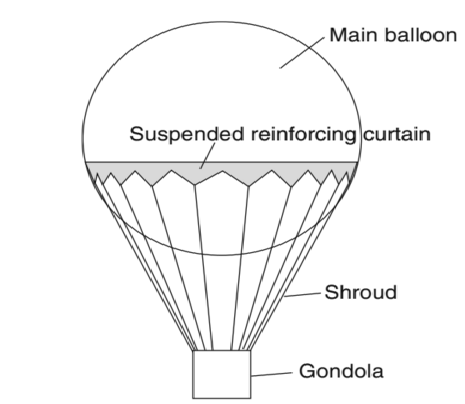
\includegraphics[width=0.5\textwidth]{figuras/balaoEsferico}
		\caption{Esquema de Balão Esférico com Fita de Carga.}
		\label{img:balaoEsferico}
	\end{figure}

	A fórmula para cálculo da tensão é a seguinte:

	$T = pr/2$ \\
	onde: \\
	\textbf{T} = tensão, \\
	\textbf{P} = pressão interna do balão, \\
	\textbf{R} = raio do balão. \\

\subsubsection{Sistema do Balão}

	Existem dois modelos de balões metereológicos empregados atualmente pela Agência Espacial Ameriacana (NASA) , o sistema Zero Pressão (ZP) e o Super-Pressão (SP).

	O sistema ZP recebe esse nome porque a pressão interna do balão é a mesma  pressão do ambiente de atuação do sistema. Na parte de baixo do envelope do balão existe pelo menos um duto que permite a saída do gás dentro do balão para o alívio da pressão interna, como é exemplificado na Figura \ref{img:maiorBalaoZeroPressao}.

	\begin{figure}[H]
		\centering
		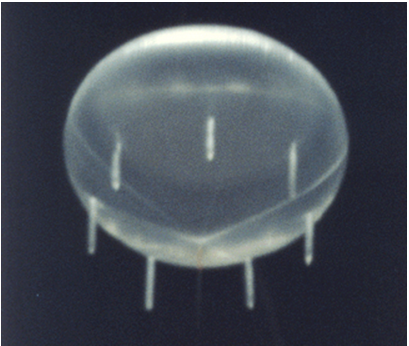
\includegraphics[width=0.5\textwidth]{figuras/maiorBalaoZeroPressao}
		\caption[Maior Balão Zero Pressão Usado pela NASA]{Maior Balão Zero Pressão Usado pela NASA~\cite{nasa1}}
		\label{img:maiorBalaoZeroPressao}
	\end{figure}

	Para esse sistema normalmente é utilizado um material com 20 micrometros de espessura para o envelope. O balão é inflado em terra e é solto na atmosfera até que a força de empuxo seja igual ao seu peso. O duto funciona de tal modo que quando a pressão interna na base do balão excede a pressão da atmosfera exterior, o duto é empurrado para fora e forma uma um cilindro que permite que parte do gás seja expelida. Quando a diferença de pressão é negativa, a pressão atmosférica empurra o duto para dentro, impedindo a entrada de ar. Com a queda de temperatura, o gás esfria e contrai-se, diminuindo o volume e consequentemente o empuxo. Em balões atmosféricos usado pela NASA, para manter a altitude constante durante a noite o balão solta pesos c, como por exemplo areia, durante esse período a quantidade de gás dentro do envelope é a mesma pois o duto se fecha quando o gás se contrai. Porém, no próximo dia, com o aumento da temperatura o gás irá se expandir, aumentando o volume e subindo mais, pois estará mais leve. Para manter uma altitude a mais constante possível, segundo a NASA, um balão desse tipo requer uma perda de 6 a 8\% de massa quando a temperatura diminui. O principal problema desse tipo de sistema é a perda de gás pelo duto aberto ao ambiente.

	O sistema SP possui a vantagem de ser completamente vedado, ou seja, não perde gás durante seu período de atividade. Por esse fato o balão tem uma pressão interna maior que a pressão externa e isso implica no aumento da espessura do envelope, normalmente cerca de 10 vezes maior que a espessura de um balão ZP (Yajima, 2009). A Figura 3 mostra a distribuição de pressão de um balão atmosférico da NASA, percebe-se que o equador do envelope é a área de maior concentração de pressão e isso inviabilizaria o uso de uma fita de carga para fixar a payload, nesse tipo de balão a payload é fixada na parte de baixo do envelope, esse fato exige que a parte de fixação seja reforçada para que o envelope não seja danificado.

	\begin{figure}[H]
		\centering
		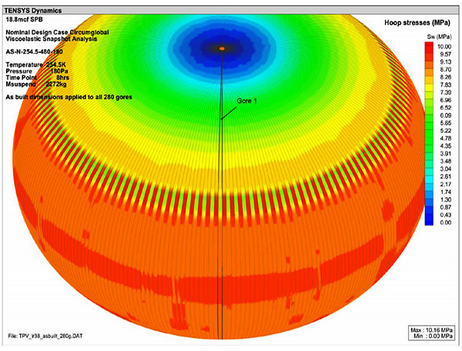
\includegraphics[width=0.5\textwidth]{figuras/distribuicaoPressao}
		\caption[Distribuição de Pressão de um Balão Super Pressão]{Distribuição de Pressão de um Balão Super Pressão~\cite{nasa2}}
		\label{img:distribuicaoPressao}
	\end{figure}

	Em linhas gerais o balão ZP é mais leve, porém possui o problema de perder gás durante sua operação. O balão SP tem a vantagem de não perder gás durante sua operação, porém é mais pesado pois precisa ter um envelope mais grosso, e não é possível o uso de uma fita de carga. Pelo fato de ser mais leve, o sistema empregado no projeto do Sistema Unificado de Monitoramento será o balão Zero Pressão. Deve-se calcular e analisar a perda diária de gás e como isso influenciará no empuxo do balão cativo.

	\subsubsection{Adaptação do Sistema de Balão para o SUM}

		Uma vez escolhido o sistema do balão deve-se adaptá-lo a um balão cativo. No caso de um balão preso ao chão o problema da perda de gás devido a variação da temperatura continua a mesma. Com o aumento da temperatura a pressão interna aumenta e pode fazer com que o gás vaze pelo duto, porém o balão não perde altitude desde que o Empuxo Líquido seja maior que zero ( o empuxo líquido é a força vertical resultante desconsiderando a tração nos cabos de sustentação). A pressão interna do balão é igual a pressão externa, com a variação da temperatura, a pressão do ar mantém-se aproximadamente constante.  Com a queda da temperatura, o gás contrai-se diminuindo o volume do balão e a pressão interna no instante de queda de temperatura é menor que a externa, desta forma o duto se fecha não permitindo a entrada de ar ou saída de gás, portanto a quantidade de matéria e a pressão dentro do envelope são aproximadamente constantes nessa fase. Usando a equação de \textit{Clapeyron}:

			$P1V1/T1 = P2V2/T2$

		com pressão constante, é possível descobrir a variação do volume do balão quando a temperatura diminui. Utilizando a base de dados do Instituto Nacional de Meteorologia (INMET) dos últimos 10 anos (entre 2005 e 2015) constata-se uma temperatura máxima média de 32ºC (305,15 K) e uma temperatura mínima média de 7.8ºC (281 K), temos o seguinte:

			 $V2/V1$ = 281/305,15  = $V2/V1$ = 0,92086

		Desta forma o volume final (V2) é cerca de 7,9% menor que o volume inicial (V1).

		Para o aumento da temperatura, ao expandir-se, o gás sai pelo duto mantendo o volume constante ( mesmo volume da queda de temperatura) , bem como a pressão aproximadamente constante, desta forma deve-se calcular a quantidade de gás perdida durante esse processo. Usando a Lei dos Gases ideais e adaptando-a para a situação temos:

			$PV = nRT$

		, como \textbf{P},\textbf{V} e \textbf{R} são constantes nesse processo temos a variação da quantidade de matéria em função da temperatura.

		$nT = cte  = n1T1 = n2T2  = n2/n1 = T1/T2$

		Sendo T1 a temperatura mais fria e T2 a temperatura mais quente, temos:

			$n2 = n1(T1/T2) = n2 = n1 (281/305,15) n2 = n1 (0,92086)$

		Logo, balão perde 7.9\% de gás por dia, podemos calcular a quantidade de matéria final após \textit{t} dias através da seguinte fórmula:

			$nf = ni (0,92086)^t$

 		onde \textbf{nf} é a quantidade de matéria final, \textbf{ni} é a quantidade de matéria inicial e \textbf{t} é o número de dias.

% subsection modelo_do_bal_o (end)

\subsection{Cálculo  do Volume do Balão} % (fold)
\label{sub:c_lculo_do_volume_do_bal_o}

	\subsubsection{Cálculo Preliminar do Volume do Balão}

	O volume do balão foi calculado primeiramente desprezando a tensão e o peso dos cabos. 	O volume do gás Hélio foi calculado da seguinte maneira:

	\begin{figure}[H]
		\centering
		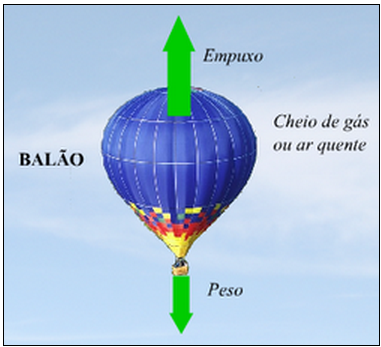
\includegraphics[width=0.5\textwidth]{figuras/corpoLivreBalao}
		\caption[Diagrama de Corpo Livre de um Balão]{Diagrama de Corpo Livre de um Balão~\cite{justino}}
		\label{img:corpoLivreBalao}
	\end{figure}

	Partindo do principio de que o volume de gás tem que gerar uma força de empuxo maior que a força peso, como mostrado na figura acima, para que o balão consiga ficar a uma certa altitude. Os cabos de apoio do balão foram desconsiderados nesse cálculo preliminar. A partir disso consideremos a seguinte fórmula para o calculo de empuxo (Munson, 2004):

	E = d\textit{ar} g V


	\textbf{V} = volume da bexiga

	\textbf{dar} = $1.225 kg/m^3$

	\textbf{MH}: massa do gás Hélio

	$MH = 0.138dar g V$

	\textbf{MM}:massa do material

 			$MM = 940 x 20e-6 x A$

	\textbf{A} = area da bexiga
	\textbf{dm} = densdidade do material = $940 kg/m^3$
	\textbf{lm} = espessura do material = 20 micrometros

	A massa da payload foi estimada em cerca de 5 kg, para margem de segurança os cálculos foram realizados com uma massa de 10 kg.

	\textbf{MP}:massa do payload

	$MP =  10kg$

	Pelo balanço de forças:

	$E = g(MH+MM+MP)$

	Substituindo 1, 2, 3 em 4, temos:

	$dar g V = g(0.138dar  V + 18,8e-3 x A + 10)$

	como trata-se de um balão esférico temos que:

	$V = 4pi r3/3 e A = 4pi r2$

	voltando a equação:

	$dar 4pi r3/3 = 0.138dar4pi r3/3 + 18,8e-3 4pi r2 +10$

	isolando e agrupando os termos semelhantes temos:

	$dar 4pi r3/3 (1 - 0.138) - 18,8e-3 4pi r2 -10 = 0$

	Substituindo os valores e usando o método de Newton para calcular as raízes de polinômios:

	$f(xi+1) = xi - f(xi) / f ’ (xi)	$

	foi obtido um valor para r = 1,4 m

	 Logo o balão teria que ter pelo menos 1,4 metros de raio. A partir desse valor calcula-se o empuxo, o peso do hélio, o peso e a quantidade de polietileno que o balão irá precisar.A tabela abaixo mostra todos os valores de forças verticais atuantes no balão. Para o cálculo do empuxo considerou-se \textbf{ar}  = $1.11166 kg/m^3$, que é a densidade do ar a 1000m de altitude. Considerou-se \textbf{h} = \textit{0.138 ar} que é a massa específica do hélio.

	 \begin{table}[H]
		\centering
		\begin{tabular}{|c|c|}
			\hline
			\rowcolor[HTML]{FFFFFF}
			{\color[HTML]{000000} \textbf{Grandezas}} & {\color[HTML]{000000} \textbf{Valores Numéricos (N)}} \\ \hline
			Empuxo                                    & 138,1                                                 \\ \hline
			Peso do Hélio                             & 19,1                                                  \\ \hline
			Peso do material do envelope              & 4,6                                                   \\ \hline
			Peso da Payload                           & 100                                                   \\ \hline
		\end{tabular}
		\caption{Forças Verticais Atuantes no Balão}
		\label{tab:forcasVerticaisAtuantes}
	\end{table}


As contas acima foram realizadas para que se tivesse uma ideia inicial do tamanho do balão e da ordem de grandeza das forças associadas.

% subsection c_lculo_do_volume_do_bal_o (end)

\subsubsection{Cálculo Real do Volume do Balão}

 O  balão irá operar em uma faixa de altura entre 20 e 25 metros em relação ao solo, porém  o mesmo será fixado no alto dos prédios da Universidade de Brasília no Campus do Gama, esses prédios têm uma altura de 10 a 12 metros dependendo do prédio. Desta forma, foram decididos os pontos de fixação e calculado o tamanho dos cabos, e concluiu-se que os cabos deveriam ter no máximo 20 metros de comprimento.
O cabo de aço escolhido tem um diâmetro de 6,4 mm e tem massa aproximada de 146 gramas por metro, um balão precisa de três cabos de sustentação de 20 metros cada. Desta forma o peso devido a massa dos cabos será:

$(C x m x g) x nc = (20 x 0.146 x 9,8 ) x 3 = 86 N$

Onde,

\textbf{C} = comprimento do cabo

\textbf{m} = massa por unidade de comprimento

\textbf{g} =  aceleração da gravidade

\textbf{nc} = número de cabos

O cabo de alimentação energética tem uma massa aproximada de 50 gramas por metro, como esse cabo não pode sofrer esforço mecânico, ele nunca  ficará tensionado e para isso seu comprimento deverá ser maior que o comprimento dos outros cabos. Para o cálculo do peso desse cabo seu comprimento será de 25 metros, procedendo da mesma forma no cálculo dos outros cabos temos:

$25 x 0,05x 9,8 = 13 N$

Portanto o peso total dos cabos será na faixa de 100 N.
Ainda existem peças que não foram levadas em consideração nessa conta como os mosquetões, sistema de estabilização entre outros. Admiti-se que essa carga extra não ultrapasse o valor de 20 N.
O volume do balão diminuirá com com o passar dos dias, visto que a quantidade de matéria diminuirá a uma taxa de 7.9\% ao dia, e para não termos que descer o balão em um pequeno intervalo de tempo dobraremos o raio do balão, ficando com um valor de 3 metros. Por margem de segurança usaremos um envelope com 60 micrometros de espessura.

A tabela abaixo mostra todos os valores de forças verticais atuantes no balão. Para o cálculo do empuxo considerou-se \textbf{ar}  = $1.11166 kg/m^3$, que é a densidade do ar a 1000m de altitude. Considerou-se $h = 0.138 ar$ que é a massa específica do hélio.

\begin{table}[H]
	\centering
	\begin{tabular}{|c|c|}
		\hline
		\rowcolor[HTML]{FFFFFF}
		{\color[HTML]{000000} \textbf{Forças}} & {\color[HTML]{000000} \textbf{Valores Numéricos (N)}} \\ \hline
		Empuxo                                 & 1232,1                                                \\ \hline
		Peso do Hélio                          & 170                                                   \\ \hline
		Peso do material do envelope           & 62,5                                                  \\ \hline
		Peso dos Cabos                         & 100                                                   \\ \hline
		Peso Extra                             & 20                                                    \\ \hline
		Peso da Payload                        & 100                                                   \\ \hline
		Empuxo Líquido                         & 780                                                   \\ \hline
	\end{tabular}
	\caption{Forças Atuantes no Balão}
	\label{tab:forcasAtuantes}
\end{table}

\subsection{Empuxo Líquido em Função do Tempo} % (fold)
\label{sub:empuxo_l_quido_em_fun_o_do_tempo}

	A força resultante gerada por um  fluido e que atua nos corpos é denominada empuxo. Esta força líquida vertical, com sentido para cima, é o resultado do gradiente de pressão (Munson, 2004). O empuxo é dado pela seguinte fórmula:

	$E = (rô)gV$ ,

	onde (rô) é a densidade do fluido, g é a aceleração da gravidade e V é o volume do fluido deslocado.
	O peso do gás utilizado é dado pela seguinte fórmula:

	$P = (rô)g V$

	Desta forma, a força (delta)F para cima do balão é

	$deltaF =  g V (rôar - rôHe)$

	DeltaF depende do volume do balão.

	 A quantidade de massa, em kilogramas, que sai pelo duto diariamente é diretamente proporcional a quantidade de matéria que sai. No caso do hélio temos:

		 $Mm = 4g/mol = Mk/n   == n = Mk/4$

	Aplicando na Eq. (2.2.4) ,temos:

	$mf = mi (0,92086)^t$ ,

	 onde mf é a massa final e mi é a massa inicial.
	Como a massa é calculada como:

	$rô g V = m$,

	temos:

	$Vf = Vi (0,92086)^t$,

	 onde \textbf{Vf} é o volume final e \textbf{Vi} é o volume inicial

	Substituindo a equação da força líquida \textbf{deltaF} nessa equação acima temos:


	$deltFf = deltaFi(0,92086)^t$

	onde deltaFf é a força líquida final e deltaFi é a força líquida inicial.

	 O empuxo líquido é dado pela soma de todas as forças verticais excluindo a força de tração nos cabos. Logo temos:

	$El = deltaF - ( Pc + Pm + Pp+Pe)$

	onde \textbf{El} é o empuxo líquido, \textbf{Pc} é o peso dos cabos, \textbf{Pm} é o peso do material do envelope, \textbf{Pp} é o peso da payload, \textbf{Pe} é o peso extra.
	Substituindo a primeira equação na segunda, podemos saber a variação do empuxo líquido no tempo. Sabendo que:

	 $Pc + Pm + Pp+Pe = 283 N$   e

	 $deltaFi = (0.862)(1,11166)(9.8)(113.1) = 1062.1 N$

	temos:

	 $El = 1062.1(0,92086)^t - 283$

	Esta equação mostra a variação do empuxo líquido em função do tempo, desta forma, é possível estimar o tempo que levará para o balão esvaziar igualando o $E_l$ a zero e isolando o tempo.

	$t = \frac{ln(283) – ln(1062.2)}{ln(0.92086} \Rightarrow t = 16 dias$

	portanto, após 16 dias o balão cairia. A figura TAL mostra o gráfico do empuxo líquido pelo tempo. O tempo ideal para reabastecer o balão com hélio é uma vez por semana, com esse tempo o balão ainda tem um empuxo líquido de 313.14 N.

	Uma observação importante é que esses cálculos realizados para predizer o comportamento do balão no tempo levam em consideração que todo dia exista uma variação térmica de cerca de 22 ºC, porém sabemos que esse fato não ocorre cotidianamente analisando os dados do INMET.


	\begin{figure}[H]
		\centering
		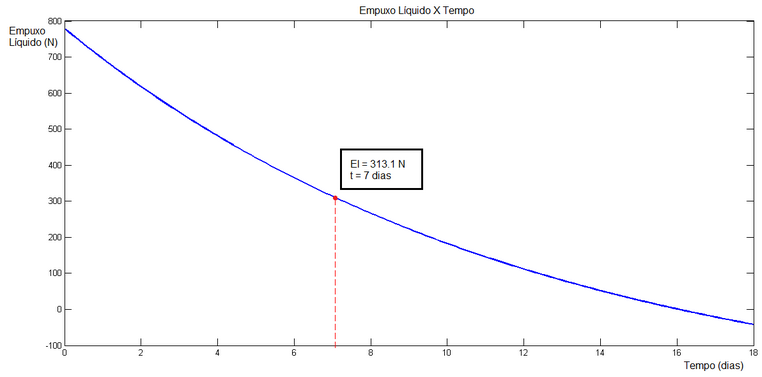
\includegraphics[width=0.8\textwidth]{figuras/empuxoLiquidoTempo}
		\caption{Gráfico de Empuxo x Tempo.}
		\label{img:empuxoLiquidoTempo}
	\end{figure}
% subsection empuxo_l_quido_em_fun_o_do_tempo (end)

\subsection{Forças no Balão} % (fold)
\label{sub:for_as_no_bal_o}

De acordo com YAJIMA(2009), a força \textbf{F} que atua no balão devido ao vento relativo tem duas componentes: A força de arrasto, que atua paralelamente a direção do vento relativo, e a força lateral, que atua perpendicular à direção do vento.
Tais forças são descritas pelas equações:

	\begin{figure}[H]
		\centering
		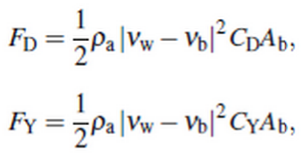
\includegraphics[width=0.5\textwidth]{figuras/equacoesArrasto}
		\caption[Numero de Reynolds para Balão]{Numero de Reynolds para Balão~\cite{yajima}}
		\label{img:equacoesArrasto}
	\end{figure}

	Onde:

	\textbf{Fd} = Força de Arrasto;

	\textbf{Fy} = Força Lateral;

	\textbf{Pa} = Densidade do Ar;

	\textbf{Cd} = Coeficiente de Arrasto;

	\textbf{Cy} = coeficiente de força lateral efetiva;

	\textbf{Ab} = Area Frontal.

	Considerando que o balão de monitoramento deve permanecer parado, podemos considerar que a velocidade do balão é nula, e a força de arrasto e força lateral se darão apenas em função da velocidade do vento.

	Para o calcula da força de arrasto e força lateral então é necessário conhecer a velocidade do vento que incidirá sobre o balão. Para determinar a velocidade do vento entramos no Banco de Dados Histórico do Instituto Nacional de Meteorologia(INMET), disponíveis no próprio site da instituição, que pode ser acessado clicando \href{www.inmet.gov.br}{AQUI}. Para termos um valor que nos desse uma margem de segurança analisamos os dados de 01/01/2005 a 01/01/2015. No período avaliado a maior velocidade do vento ocorrida no DF registrada foi de 17 m/s.

	O Coeficiente de Arrasto e o coeficiente de força lateral está diretamente relacionado ao número de Reynolds. O número de Reynolds é um número adimensional usado em mecânica dos fluidos para o cálculo do regime de escoamento de determinado fluido dentro de um tubo ou sobre uma superfície (BIRD, 2004).

	Segundo YAJIMA(2009), o número de Reynolds para um balão é dado pela equação:

	\begin{figure}[H]
		\centering
		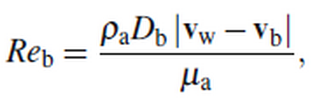
\includegraphics[width=0.5\textwidth]{figuras/equacaoNumeroDeRey}
		\caption{Numero de Reynolds para Balão~\cite{yajima}}
		\label{img:equacaoNumeroDeRey}
	\end{figure}

	Onde:

	\textbf{Reb} = Número de Reynolds;

	\textbf{Db} = Diâmetro do Balão;

	\textbf{Vw} = Velocidade do Vento;

	\textbf{Vb} = Velocidade do Balão;

	\textbf{“Mí”a} = coeficiente de viscosidade do Ar .

	Considerando que o balão terá um diâmetro de 6m e a Brasília se encontra a uma altitude próxima a 1000m acima do nível do Mar. Temos que:

	Densidade do Ar a 1km de altitude: “Rô”a = $1,11166 Kg/m^3$ - Tabela de atmosfera padrão  (BIRD,2004)

	Diâmetro do Balão: 6m

	Velocidade máxima do vento observada: 17 m/s

	Viscosidade do Ar : 0,01813 mPa.s (BIRD,2004)

	Logo:

	Reb = $(1.11166 kg/m^3 X 6m X 17 m/s) / 0,01813 x 10^(-3) Pa.s$

	$Reb = 6.354 x 10^6$

	A Tabela a seguir mostra o coeficiente de arrasto do balão em função do número de Reynolds do fluido e do formato do balão. Para o número de Reynolds da ordem de 6 x 106  temos um coeficiente de arrasto de aproximadamente 0,2.

	\begin{figure}[H]
		\centering
		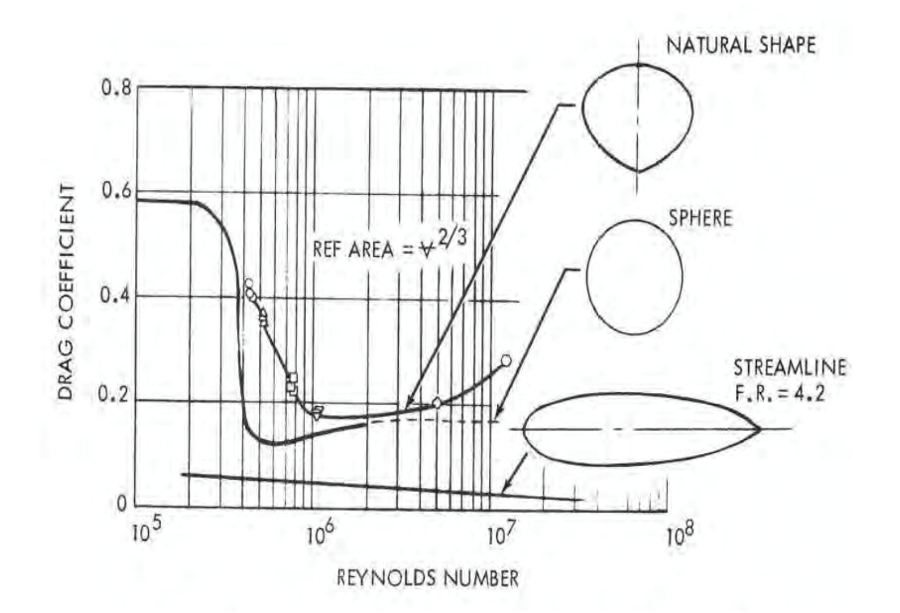
\includegraphics[width=0.5\textwidth]{figuras/coeficienteArrasto}
		\caption{Coeficiente de Arrasto x Número de Reynolds}
		\label{img:coeficienteArrasto}
	\end{figure}

	Tendo em mão esses valores podemos então calcular a força máxima de arrasto que o balão estará sujeito. Temos que:

	\begin{figure}[H]
		\centering
		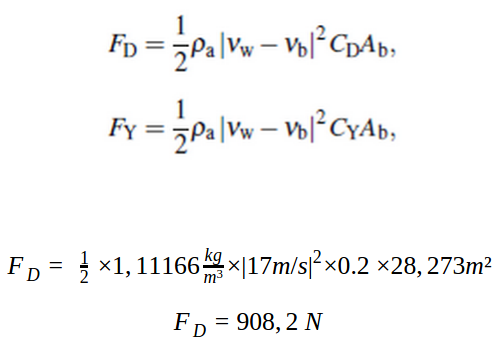
\includegraphics[width=0.5\textwidth]{figuras/formulasCoeficienteArrasto}
		\caption{}
		\label{img:formulasCoeficienteArrasto}
	\end{figure}


	O coeficiente de força lateral efetiva para um balão que se encontra estacionário é de 0.18 (FERGUSON,1981). Podemos observar que nas duas equações este é o único valor que se altera, logo temos que:

	Fy=817,38 N

	Temos então que sobre o Balão atuaram as seguintes forças:

	Força de Arrasto: 908,2 N

	Força Lateral: 817,38 N

	Força de Empuxo: 800 N

	O que nos dá uma força resultante de:

	$\textbf{FD}= \sqrt{908,22+ 817,382+8002N}$

	\textbf{FD}=1460,458 N

\subsection{Posicionamento dos cabos}

	A posição em relação ao balão a qual os cabos estarão fixados possui grande importância, pois o mal posicionamentos deles poderá levar o balão a uma condição de instabilidade, logo prejudicando o monitoramento. O balão será fixado por três cabos, cuja  configuração é mostrada pela figura \ref{img:coordcabos}.

	\begin{figure}[H]
		\centering
		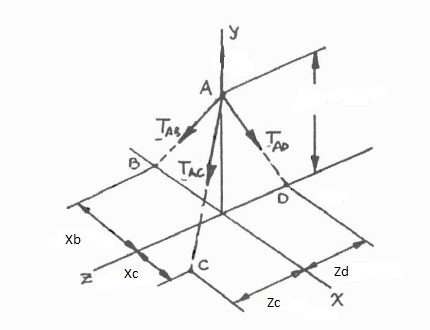
\includegraphics[width=0.8\textwidth]{figuras/coorcabo}
		\caption{Coordenadas do cabo \cite{beer}}
		\label{img:coordcabos}
	\end{figure}

	Serão utilizados cinco balões, que serão posicionados de acordo com a seguinte configuração: dois balões estarão em cima da Unidade de Ensino e Docência (UED) e outros dois balões no terraço na Unidade Acadêmica (UAC). Para estes balões, dois cabos estarão fixados no topo do prédio (pontos B e C na figura) e um terceiro cabo será preso numa haste (pontos C) de 10 m de altura que ficará a uma determinada distância dos prédios. O quinto balão ficará posicionado em cima do restaurante universitário (RU), onde dois cabos serão fixados em cima do RU (pontos B e D) e o terceiro cabo será preso a uma haste (ponto C) que possui a altura do restaurante universitário.

	Para que o balão fique em uma posição de equilíbrio o sistema de equações abaixo deve ser respeitado.

	$\left [ - \frac{x_{b}}{L_{B}}T_{AC} - \frac{Y-Y_{p}}{L_{b}}T_{AB}0 - \frac{x_{c}}{L_{C}}T_{AB} - \frac{Y-Y_{h}}{L_{C}}T_{AC} \frac{Z_{c}}{L_{C}}T_AC0 \right ]$

	Onde:\\
$L_{B}$: Comprimento do cabo do ponto A até o ponto B\\
$L_{C}$: Comprimento do cabo do ponto A até o ponto C\\
$L_{D}$: Comprimento do cabo do ponto A até o ponto D\\
$E_{L}$: Empuxo líquido\\
$F_{D}$: Força de arrasto\\
$F_{dx}$: Componente - x da força aerodinâmica\\
$F_{dz}$: Componente – z da força aerodinâmica\\
$Y$: Altura do balão\\
$Y_{p}$: Altura do prédio\\
$Y_{h}$: Altura da haste\\

A melhor abordagem para resolver este sistema é definir aonde estarão fixados os cabos ($x_{b}$, $x_{c}$, $z_{c}$, $z_{d}$) e estabelecer o comprimento de cada cabo ($L_{B}$, $L_{C}$, $L_{D}$), logo as incógnitas serão as forças em cada cabo ($T_{AB}$, $T_{AC}$, $T_{AD}$). Portanto, deve-se escolher as posições dos cabos que forneçam valores de forças fisicamente possíveis. Outro ponto importante é que a força do cabo que é fixado na haste seja bem inferior em relação as forças dos cabos preso aos prédios, logo será necessário o uso de uma haste com simples resistência a tração, ao invés de uma haste com boas propriedades mecânica no então de custo elevado.

	Para as condições de projeto:

	O empuxo líquido, $E_{L}$, foi calculado anteriormente, o seu valor é de 800 N. A forca de arrasto, $F_{D}$ é de aproximadamente 880 N. Portando a força total exercida nos cabos é de aproximadamente 1200 N. Assume-se que a força de arrasto é dividida igualmente entre a componente x e z: $F_{dx}$ = 440 N e $F_{dz}$ = 440 N.

	\begin{itemize}
		\item  Altura do balão = 10 m
 		\item Altura do UED = 10 m
 		\item Altura do UAC = 10 m
 		\item Altura do RU = 4 m
 		\item Altura da haste = 10 m
	\end{itemize}

\begin{table}[H]
\centering
\begin{tabular}{l|l|l|l|l|l|l|l|l|l|l|}
\cline{2-11}
 & $X_{b}$ m & $X_{c}$ m & $Z_{c}$ m & $Z_{d}$ m & $L_{b}$ m & $L_{c}$ m & $L_{D}$ m & $\Theta _{B}$ & $\Theta _{C}$ & $\Theta _{D}$ \\ \hline
\multicolumn{1}{|l|}{UED} & 18,0 & 5,0 & 10,0 & 18,0 & 23,5 & 18,7 & 23,5 & 39,8 & 45,0 & 39,8 \\ \hline
\multicolumn{1}{|l|}{UAC} & 18,0 & 5,0 & 10,0 & 18,0 & 23,5 & 18,7 & 23,5 & 39,8 & 45,0 & 39,8 \\ \hline
\multicolumn{1}{|l|}{RU} & 25,0 & 5,0 & 15,0 & 25,0 & 32,7 & 26,3 & 32,7 & 40,3 & 46,4 & 40,3 \\ \hline
\end{tabular}
\caption{Posição, comprimento e ângulo dos cabos}
\label{tab:composangcabos}
\end{table}

Portanto, para os balões presentes no UED e UAC, o cabo fixado na haste ficará aproximadamente a 12 metros do prédio, e o cabos que estão presos no terraço estão a aproximadamente 18 metros do balão. Para o balão posicionado no RU, o cabo na haste estará a 16 metros do prédio, e os cabos fixados no topo do prédio a 25 metros do balão.

\begin{table}[H]
\centering
\begin{tabular}{l|l|l|l|}
\cline{2-4}
 & $T_{AB}$ [N] & $T_{AC}$ [N] & $T_{AD} [N]$ \\ \hline
\multicolumn{1}{|l|}{UED} & 588,53 & 45,35 & 604,31 \\ \hline
\multicolumn{1}{|l|}{UAC} & 588,53 & 45,35 & 604,31 \\ \hline
\multicolumn{1}{|l|}{RU} & 585,13 & 42,28 & 606,14 \\ \hline
\end{tabular}
\caption{ Módulo das tensões}
\label{table:modTensoes}
\end{table}

\subsection{Sustentação do SUM}

O Balão Cativo será fixado em três pontos diferentes para que seja garantida sua estabilidade considerando ventos laterais de qualquer direção, adotou-se o modelo de balão de zero pressão de formato esférico preenchido com gás hélio. No caso dos balões de zero pressão há uma perda diária do volume de gás de cerca de 8\%. O volume de gás hélio no balão será de 113m$^{3}$ e, considerando as perdas diárias, estima-se que a cada sete dias haverá a necessidade de  efetuar uma reposição desse gás para garantir o bom funcionamento do monitoramento do estacionamento, onde o empuxo gerado pelo gás seja suficiente para manter uma altitude de 20m.

A fixação será adaptada para cada um dos balões, pois como estarão em lugares distintos e estratégicos estudaremos cada um dos três pontos de fixação. A manutenção do balão será feita em solo, por exemplo: no caso de reposição do gás, na reparação de algum item interno da payload e etc. Para tal iremos utilizar dois motores elétricos para puxar o balão até o solo, os motores estarão fixos no chão onde será definido o local onde o cabo de sustentação será fixado, ou seja, o cabo de sustentação estará sendo regulado pelo motor.

De acordo com cálculos realizados previamente, a força resultante do balão será de aproximadamente de 6.4 KN. A partir destas informações, escolhemos o motor vendido pela empresa Bremen com a capacidade de 7240 Kg, potência de 4500W, 12V de tensão e pesando 52,5 Kg. A seguir encontra-se a tabela de motores vendidos pela mesma empresa.

\begin{figure}[H]
	\centering
	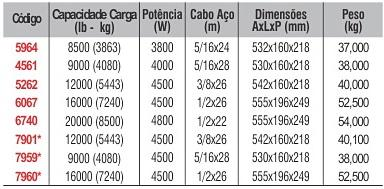
\includegraphics[width=0.8\textwidth]{figuras/tabelamotor}
	\caption{Tabela ilustrativa dos tipos de motores disponíveis \cite{bremem}}
	\label{img:tabelamotor}
\end{figure}

\begin{figure}[H]
	\centering
	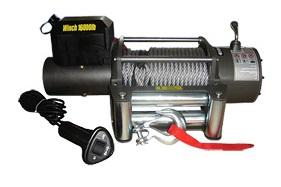
\includegraphics[width=0.8\textwidth]{figuras/modelodemotoreletrico}
	\caption{Modelo de motor elétrico escolhido \cite{bremem}}
	\label{img:motorescolhido}
\end{figure}

A Figura \ref{img:motorescolhido} ilustra como será o motor. Para este motor será efetuada uma simples adaptação no cabo, onde será substituído o cabo de fábrica pelo cabo de aço classe 8x19 – Alma de Fibra com diâmetro de 6,4 mm. A alteração foi necessária em consideração ao peso do cabo, pois o mesmo é mais leve em relação ao cabo de aço comum, e também possui boas propriedades mecânicas como mostrado na tabela a seguir:

\begin{figure}[H]
	\centering
	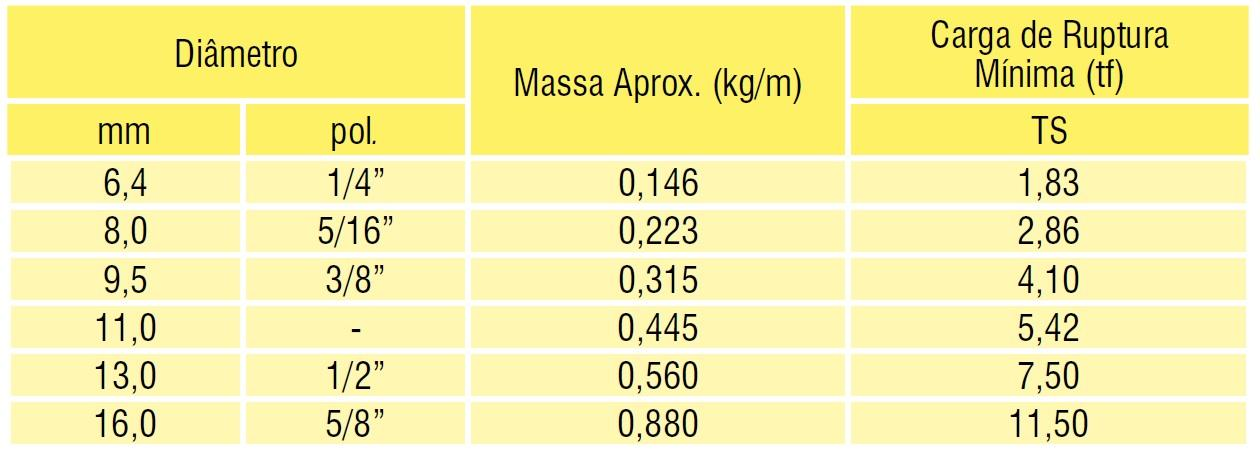
\includegraphics[width=0.8\textwidth]{figuras/tabelacabo}
	\caption{Propriedade do cabo Alma de Fibra. \cite{acrocabo}}
	\label{img:motorescolhido}
\end{figure}
